% -------------------------------------------------------------------
\chapter{Leituras de SO2 adquiridas pelo sensor SO2-B4}\label{apendix:so2-readings}
% -------------------------------------------------------------------

Para a medição de \acrshort{so2} foram utilizados dois sensores do modelo SO2-B4. As Figuras \ref{fig:data-so2-1-raw} e \ref{fig:data-so2-2-raw} mostram as séries temporais dos sensores depois de removidos os valores fora de intervalo. Observa-se que ambos sensores sofreram seguidas alterações no valor de linha base (Figuras \ref{fig:data-rebase-so2-1} e \ref{fig:data-rebase-so2-1}), sendo difícil aproveitar algum período de dados úteis. As distribuições das leituras dos sensores também não apresentaram um formato log-normal como se observa nos histogramas das leituras dos sensores mostrados nas Figuras \ref{fig:data-so2-1-preproc-hist} e \ref{fig:data-so2-2-preproc-hist}. Por esses motivos os dados desses sensores não foram considerados para análise no trabalho.

\begin{figure}[h!]
    \centering
    \caption{Série temporal dos sensores de \acrshort{so2} modelo SO2-B4}
    \begin{subfigure}{0.495\textwidth}
        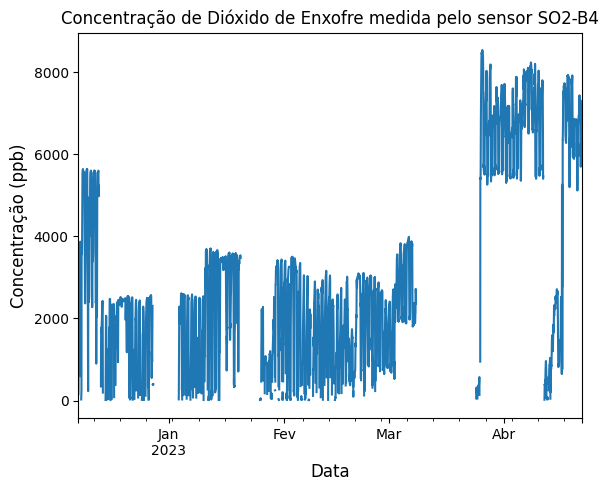
\includegraphics[width=\textwidth]{aftertext/Leituras SO2/raw-so2-b4-1.png}
        \caption{Série temporal do sensor 1 depois de remover valores fora de intervalo}
        \label{fig:data-so2-1-raw}
    \end{subfigure}
    \hfill
    \begin{subfigure}{0.495\textwidth}
        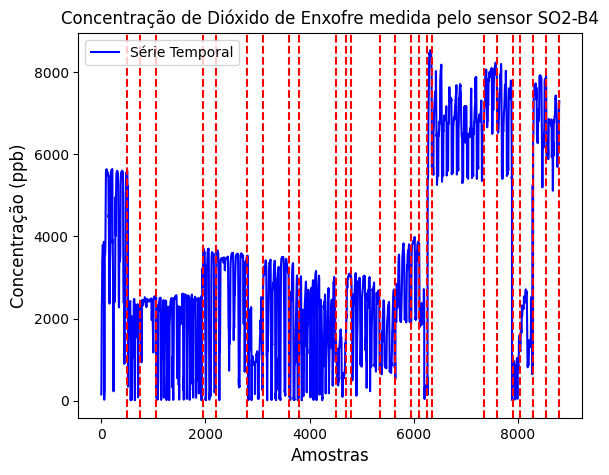
\includegraphics[width=\textwidth]{aftertext/Leituras SO2/rebase-so2-b4-1.png}
        \caption{Pontos de alteração da linha base no sensor 1 detectados pelo algoritmo \acrshort{pelt}}
        \label{fig:data-rebase-so2-1}
    \end{subfigure}
    \hfill
    \begin{subfigure}{0.495\textwidth}
        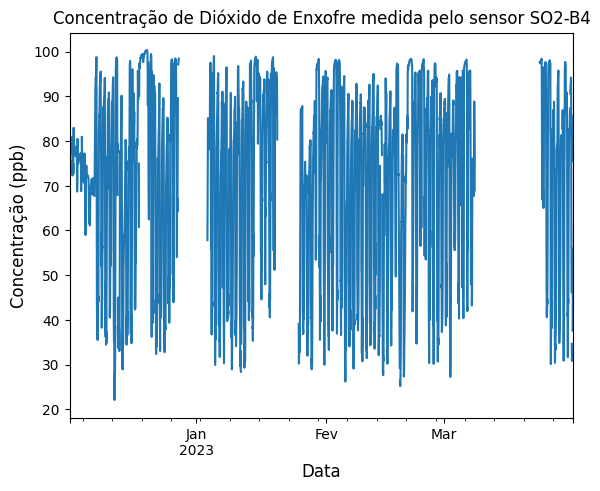
\includegraphics[width=\textwidth]{aftertext/Leituras SO2/raw-so2-b4-2.png}
        \caption{Série temporal do sensor 2 depois de remover valores fora de intervalo}
        \label{fig:data-so2-2-raw}
    \end{subfigure}
    \hfill
    \begin{subfigure}{0.495\textwidth}
        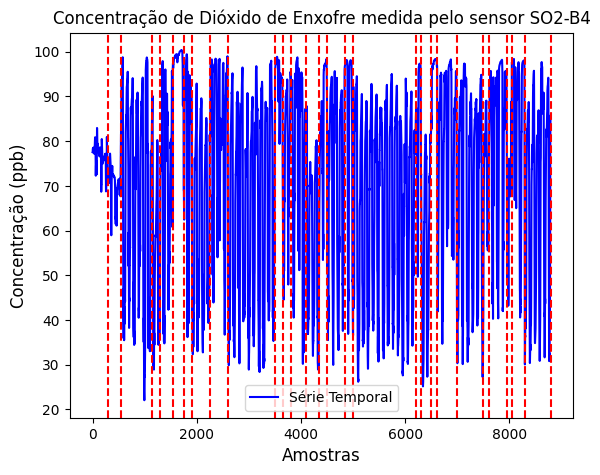
\includegraphics[width=\textwidth]{aftertext/Leituras SO2/rebase-so2-b4-2.png}
        \caption{Pontos de alteração da linha base no sensor 2 detectados pelo algoritmo \acrshort{pelt}}
        \label{fig:data-rebase-so2-2}
    \end{subfigure}
    \label{fig:data-so2-raw-and-pelt}
\end{figure}

\begin{figure}[h]
    \centering
    \caption{Histogramas das leituras dos sensores SO2-B4}
    \begin{subfigure}{0.495\textwidth}
        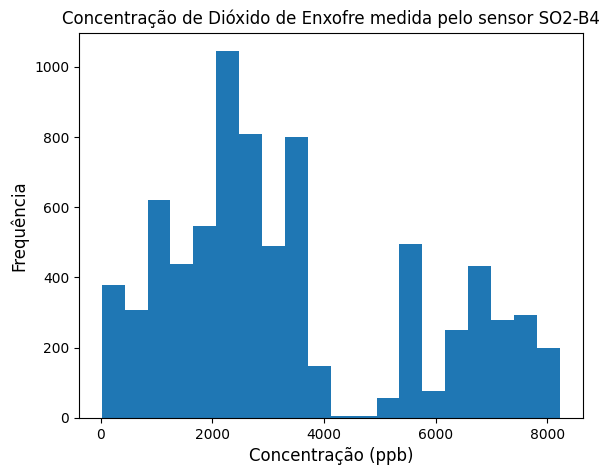
\includegraphics[width=\textwidth]{aftertext/Leituras SO2/preproc-hist-so2-b4-1.png}
        \caption{Histograma das leituras do sensor 1 SO2-B4}
        \label{fig:data-so2-1-preproc-hist}
    \end{subfigure}
    \hfill
    \begin{subfigure}{0.495\textwidth}
        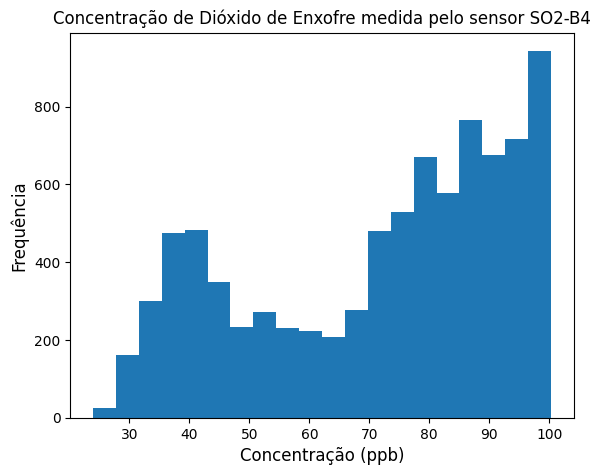
\includegraphics[width=\textwidth]{aftertext/Leituras SO2/preproc-hist-so2-b4-2.png}
        \caption{Histograma das leituras do sensor 2 SO2-B4}
        \label{fig:data-so2-2-preproc-hist}
    \end{subfigure}
\end{figure}